\documentclass[a4paper,12pt]{article}
\usepackage[utf8]{inputenc}
\usepackage[german]{babel}
\usepackage{amsmath,amssymb,amsthm}
\usepackage{geometry}
\usepackage{graphicx}
\usepackage{xcolor}
\usepackage{booktabs}
\usepackage{array}
\usepackage{longtable}
\usepackage{hyperref}
\usepackage{caption}
\usepackage{subcaption}
\usepackage{float}
\usepackage{microtype}
\usepackage{parskip}
\usepackage{enumitem}
\usepackage{mdframed}
\usepackage{fancyhdr}
\usepackage{titlesec}
\usepackage{tocloft}
\usepackage{mathtools}
\usepackage{cleveref}
\usepackage{siunitx}
\usepackage{microtype}


\geometry{margin=2.5cm}
\setlist[itemize,1]{label=--}

\definecolor{primaryblue}{HTML}{0F52BA}
\definecolor{secondarygreen}{HTML}{048A81}
\definecolor{accentblue}{HTML}{54C6EB}
\definecolor{warnred}{HTML}{EF6461}
\definecolor{lightbg}{HTML}{E8F1F2}
\definecolor{darkgray}{HTML}{374151}

% -------------------------------------------------------
% Hyperref
% -------------------------------------------------------
\hypersetup{
  colorlinks=true,
  linkcolor=primaryblue,
  citecolor=secondarygreen,
  urlcolor=secondarygreen
}

\theoremstyle{definition}
\newtheorem{theorem}{Theorem}[section]
\newtheorem{lemma}[theorem]{Lemma}
\newtheorem{korollar}[theorem]{Korollar}
\newtheorem{proposition}[theorem]{Proposition}
\newtheorem{definition}[theorem]{Definition}
\newtheorem{bemerkung}[theorem]{Bemerkung}
\newtheorem{beispiel}[theorem]{Beispiel}

% -------------------------------------------------------
% SI-Einheiten
% -------------------------------------------------------
\sisetup{
  locale=DE,
  per-mode=symbol,
  detect-weight=true
}

% -------------------------------------------------------
% Metadaten
% -------------------------------------------------------

\title{\bfseries Physikalische Modellierung und bautechnische Analyse von Feuchtesch\"aden an Mauerwerk und Kellerkonstruktionen}
\author{Stephan Epp}
\date{26. April 2026}

% =======================================================
\begin{document}
% =======================================================

\maketitle
\tableofcontents
\newpage

% =======================================================
\section{Einleitung}
% =======================================================
Feuchtesch\"aden an Au\ss{}enw\"anden und in Kellergeschossen z\"ahlen zu den
h\"aufigsten und kostspieligsten Schadensf\"allen im Bauwesen. Die vorliegende
Arbeit entwickelt eine formal-physikalische Grundlage zur Beschreibung,
Pr\"avention und Sanierung von Durchfeuchtungserscheinungen in Mauerwerk und
Betonkonstruktionen. Ausgehend von der Young-Laplace-Gleichung f\"ur
kapillaren Transport, den Fick'schen Diffusionsgesetzen und der thermody\-namischen
Taupunktanalyse nach Magnus werden Feuchteausbreitungsmodelle hergeleitet
und deren analytische L\"osungen angegeben. Der Glasersche Diffusionsansatz
wird auf mehrschichtige Kellerw\"ande angewendet. Das Schimmelwachstumsrisiko
wird quantitativ nach dem Viitanen-Modell bewertet. Sechs hochaufl\"osende
Abbildungen veranschaulichen die Ergebnisse numerisch. Abschlie\ss{}end werden
kurz-, mittel- und langfristige Pr\"aventions- und Sanierungsma\ss{}nahmen
systematisch verglichen und hinsichtlich Effektivit\"at sowie Wirtschaftlichkeit
bewertet. Der Ausblick skizziert offene Forschungsfragen und zuk\"unftige
Entwicklungspotenziale in Simulation, Sensorik und Materialentwicklung.

Durchfeuchtungserscheinungen in Geb\"auden verursachen in Deutschland j\"ahrlich
Schadenskosten von mehreren Milliarden Euro. Laut Statistiken des Gesamtverbands
der Deutschen Versicherungswirtschaft (GDV) entfallen rund 30\,\% aller
Geb\"audesch\"aden auf Wasser- und Feuchtigkeitsprobleme. Insbesondere Kellergeschosse
sind aufgrund ihrer direkten Erdber\"uhrung und der h\"aufig mangelhaften historischen
Abdichtung besonders gef\"ahrdet.

Nasse W\"ande und feuchte Keller sind jedoch kein schicksalhaftes Ph\"anomen --
sie folgen klar beschreibbaren physikalischen Gesetzm\"a\ss{}igkeiten und k\"onnen
durch gezielte Ma\ss{}nahmen verhindert oder behoben werden. Das
Verst\"andnis der zugrunde liegenden Transportmechanismen -- Kapillarit\"at,
Dampfdiffusion, Konvektion und W\"armeleitung -- bildet die unverzichtbare
Basis f\"ur jede Planungs- und Sanierungsentscheidung.

\subsection{Motivation und wissenschaftliche Relevanz}

Die wachsende Klimavariabilit\"at mit intensiveren Starkregenereignissen
und h\"oheren Grundwasserst\"anden erh\"oht die Belastung bestehender
Geb\"audesubstanz erheblich. Gleichzeitig wird der Energieeffizienz-
anspruch im Rahmen der Geb\"audesanierung nach GEG (Geb\"audeenergiegesetz)
immer strenger, was h\"aufig zu bauphysikalisch problematischen Zust\"anden
f\"uhrt, wenn W\"armed\"ammung ohne gleichzeitige Feuchtebetrachtung
aufgebracht wird.

\subsection{Ziele der Arbeit}

Die vorliegende Arbeit verfolgt folgende Ziele:
\begin{enumerate}
  \item Formale physikalische Herleitung der relevanten Transportgleichungen.
  \item Analytische L\"osung des Feuchtetransportproblems in Wandquerschnitten.
  \item Quantitative Bewertung des Schimmelrisikos mittels Viitanen-Modell.
  \item Systematischer Vergleich pr\"aventiver und sanierender Ma\ss{}nahmen.
  \item Entwicklung eines Entscheidungsrahmens f\"ur Planung und Sanierung.
\end{enumerate}

\subsection{Aufbau der Arbeit}

Nach der Darstellung der physikalischen Grundlagen
(\cref{sec:grundlagen}) werden die Ursachen von
Feuchtesch\"aden klassifiziert (\cref{sec:ursachen}).
Abschnitt~\ref{sec:pravention} behandelt pr\"aventive Ma\ss{}nahmen,
Abschnitt~\ref{sec:sanierung} Sanierungsstrategien bei bestehenden
Sch\"aden. Den Abschluss bilden Schlussfolgerungen (\cref{sec:fazit})
und ein ausf\"uhrlicher Ausblick (\cref{sec:ausblick}).

\textbf{Schlagw\"orter:} Kapillarit\"at, Feuchtediffusion, Glaserdiagramm,
Taupunkt, Schimmelwachstum, Kellersanierung, Perimeterd\"ammung, Young-Laplace.

% =======================================================
\section{Physikalische Grundlagen des Feuchtetransports}
\label{sec:grundlagen}
% =======================================================

\subsection{Kapillarit\"at und die Young-Laplace-Gleichung}

Die Kapillarit\"at beschreibt den spontanen Aufstieg von Fl\"ussigkeiten
in engen Poren infolge von Oberfl\"achenspannungskr\"aften. Sie ist der
prim\"are Mechanismus f\"ur den aufsteigenden kapillaren Feuchtetransport
in erdber\"uhrtem Mauerwerk.

\begin{definition}[Kapillardruck nach Young-Laplace]
\label{def:young-laplace}
F\"ur eine zylindrische Pore mit Radius $r$, Oberfl\"achenspannung
$\gamma$ der Fl\"ussigkeit und Kontaktwinkel $\theta$ an der Feststoff-
Fl\"ussigkeits-Grenzfl\"ache gilt f\"ur den Kapillardruck:
\begin{equation}
  \Delta p = \frac{2\,\gamma\,\cos\theta}{r}.
  \label{eq:young-laplace}
\end{equation}
\end{definition}

\begin{lemma}[Kapillare Steigh\"ohe]
\label{lem:steihoehe}
Aus dem Gleichgewicht zwischen Kapillardruck und hydrostatischem Druck
$\rho\,g\,h_k$ ergibt sich die maximale Steigh\"ohe:
\begin{equation}
  h_k = \frac{2\,\gamma\,\cos\theta}{\rho\,g\,r}.
  \label{eq:steihoehe}
\end{equation}
\end{lemma}

\begin{proof}
Im hydrostatischen Gleichgewicht gilt $\Delta p = \rho\,g\,h_k$.
Einsetzen von \cref{eq:young-laplace} liefert unmittelbar
$\rho\,g\,h_k = 2\gamma\cos\theta/r$, woraus
\cref{eq:steihoehe} folgt. 
\end{proof}

\begin{bemerkung}
F\"ur Wasser bei \SI{20}{\celsius} gilt $\gamma = \SI{0.0728}{N/m}$
und $\rho = \SI{998}{kg/m^3}$. Bei einem Kontaktwinkel $\theta = 0°$
(vollst\"andige Benetzung, typisch f\"ur Ziegelmauerwerk) und einem
Porenradius $r = \SI{10}{\micro m}$ ergibt sich eine Steigh\"ohe von
\begin{equation*}
  h_k = \frac{2 \times 0{,}0728}{998 \times 9{,}81 \times 10^{-5}}
      \approx \SI{1.49}{m}.
\end{equation*}
In Mauerwerk mit Kapillarporenradien im Bereich \SIrange{0.1}{10}{\micro m}
k\"onnen damit Steigh\"ohen von mehreren Metern auftreten.
\end{bemerkung}

\Cref{fig:kapillardruck} veranschaulicht den Kapillardruck und
die Steigh\"ohe als Funktion des Porenradius f\"ur verschiedene
Kontaktwinkel.

\begin{figure}[H]
  \centering
  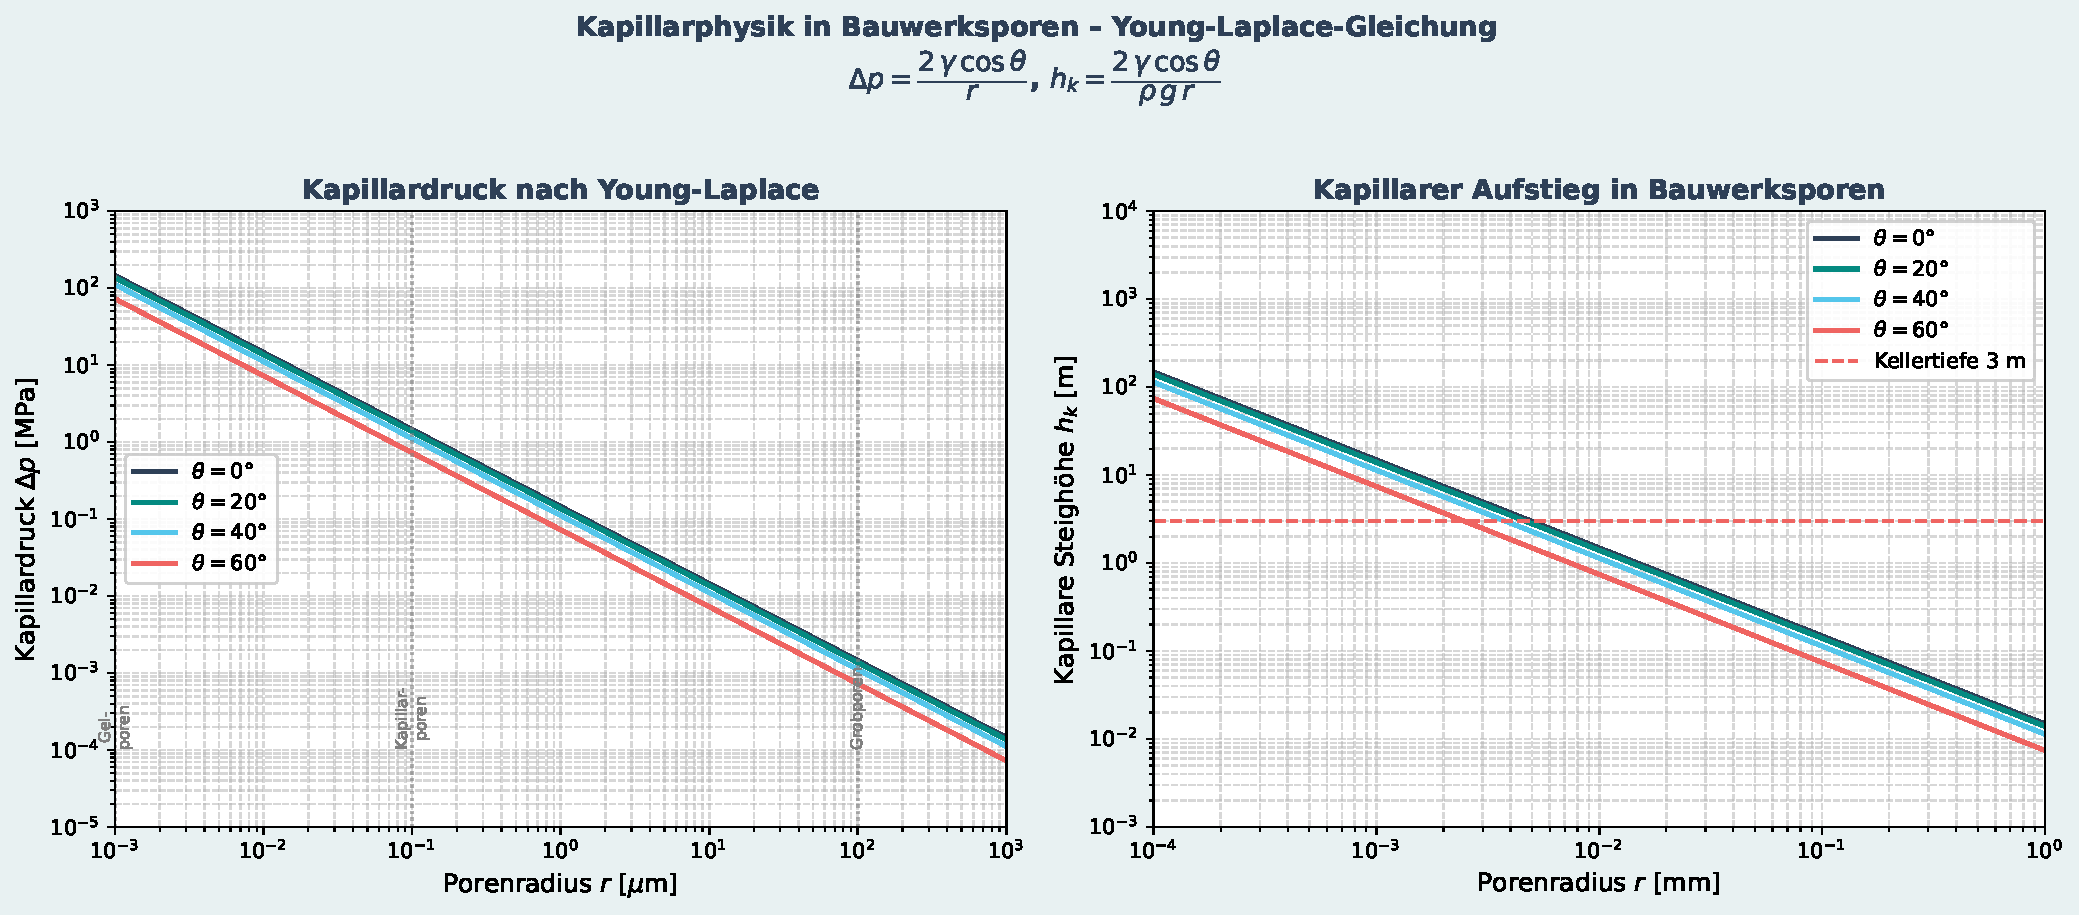
\includegraphics[width=\linewidth]{plot1_kapillardruck.pdf}
  \caption{%
    \textbf{Kapillarphysik in Bauwerksporen.}
    \textit{Links:} Kapillardruck $\Delta p$ nach der Young-Laplace-Gleichung
    als Funktion des Porenradius $r$ f\"ur Kontaktwinkel
    $\theta \in \{0°,\,20°,\,40°,\,60°\}$. Die vertikalen Linien markieren
    typische Porengr\"o\ss{}enbereiche in Baustoffen (Gelporen, Kapillarporen,
    Grobporen). \textit{Rechts:} Kapillare Steigh\"ohe $h_k$ nach
    \cref{lem:steihoehe}; die gestrichelte Linie bei \SI{3}{m} repr\"asentiert
    eine typische Kellertiefe als Referenz.}
  \label{fig:kapillardruck}
\end{figure}

\subsection{Feuchtediffusion -- Fick'sche Gesetze}

Neben dem kapillaren Fl\"ussigtransport ist die Dampfdiffusion ein weiterer
wesentlicher Feuchtetransportmechanismus. Sie wird durch die Fick'schen
Gesetze beschrieben.

\begin{definition}[Erstes Fick'sches Gesetz -- station\"are Diffusion]
Der Diffusionsstromdichte-Vektor $\mathbf{j}$ ist proportional zum
negativen Konzentrationsgradienten:
\begin{equation}
  \mathbf{j} = -D\,\nabla u,
  \label{eq:fick1}
\end{equation}
mit dem Diffusionskoeffizienten $D$ [\si{m^2/s}] und der
normierten Feuchtekonzentration $u$ [-].
\end{definition}

\begin{definition}[Zweites Fick'sches Gesetz -- instation\"are Diffusion]
Die zeitliche \"Anderung der Feuchtekonzentration gehorcht der
partiellen Differentialgleichung:
\begin{equation}
  \frac{\partial u}{\partial t} = D\,\Delta u = D\,\nabla^2 u.
  \label{eq:fick2}
\end{equation}
Im eindimensionalen Fall (Wandquerschnitt, $x \in [0,L]$) vereinfacht
sich dies zu:
\begin{equation}
  \frac{\partial u}{\partial t} = D\,\frac{\partial^2 u}{\partial x^2}.
  \label{eq:fick2_1d}
\end{equation}
\end{definition}

\begin{theorem}[Analytische L\"osung der 1D-Diffusionsgleichung]
\label{thm:fourier}
Sei $u(x,t)$ die L\"osung von \cref{eq:fick2_1d} auf $[0,L]$ mit
den Randbedingungen $u(0,t)=1$ (feuchte Au\ss{}enseite) und $u(L,t)=0$
(trockene Innenseite) sowie der Anfangsbedingung $u(x,0)=0$. Dann gilt:
\begin{equation}
  u(x,t) = \underbrace{\left(1 - \frac{x}{L}\right)}_{\text{station\"arer Anteil}}
  + \sum_{n=1}^{\infty}
  \frac{-2}{n\pi}\,(-1)^n\,\sin\!\left(\frac{n\pi x}{L}\right)
  \exp\!\left(-D\,\frac{n^2\pi^2}{L^2}\,t\right).
  \label{eq:fourier_loesung}
\end{equation}
\end{theorem}

\begin{proof}
Wir zerlegen $u = u_{\mathrm{stat}} + v$ mit station\"arem Anteil
$u_{\mathrm{stat}}(x) = 1 - x/L$ (L\"osung von $u''=0$ mit den RB)
und transientem Anteil $v(x,t)$ mit homogenen Randbedingungen
$v(0,t)=v(L,t)=0$ und $v(x,0) = -(1-x/L)$.

Die Differentialgleichung $v_t = D\,v_{xx}$ mit homogenen RB wird durch
den Separationsansatz $v(x,t)=X(x)\,T(t)$ gel\"ost. Die Eigenfunktionen
sind $X_n(x) = \sin(n\pi x/L)$ mit Eigenwerten $\lambda_n = (n\pi/L)^2$.
Der Zeitanteil ist $T_n(t)=\exp(-D\lambda_n t)$.

Die Fourierkoeffizienten der Anfangsbedingung ergeben sich als:
\begin{equation*}
  c_n = \frac{2}{L}\int_0^L \!-(1-\tfrac{x}{L})\,\sin\!\tfrac{n\pi x}{L}\,\mathrm{d}x
      = \frac{-2}{n\pi}(-1)^n.
\end{equation*}
Addition ergibt \cref{eq:fourier_loesung}. 
\end{proof}

Die charakteristische Diffusionszeit ist:
\begin{equation}
  \tau_D = \frac{L^2}{\pi^2\,D}.
  \label{eq:tauD}
\end{equation}

\Cref{fig:diffusion} zeigt die Feuchteausbreitung nach \cref{thm:fourier}
f\"ur eine \SI{36}{cm} dicke Betonwand mit
$D = \SI{3.5e-10}{m^2/s}$.

\begin{figure}[H]
  \centering
  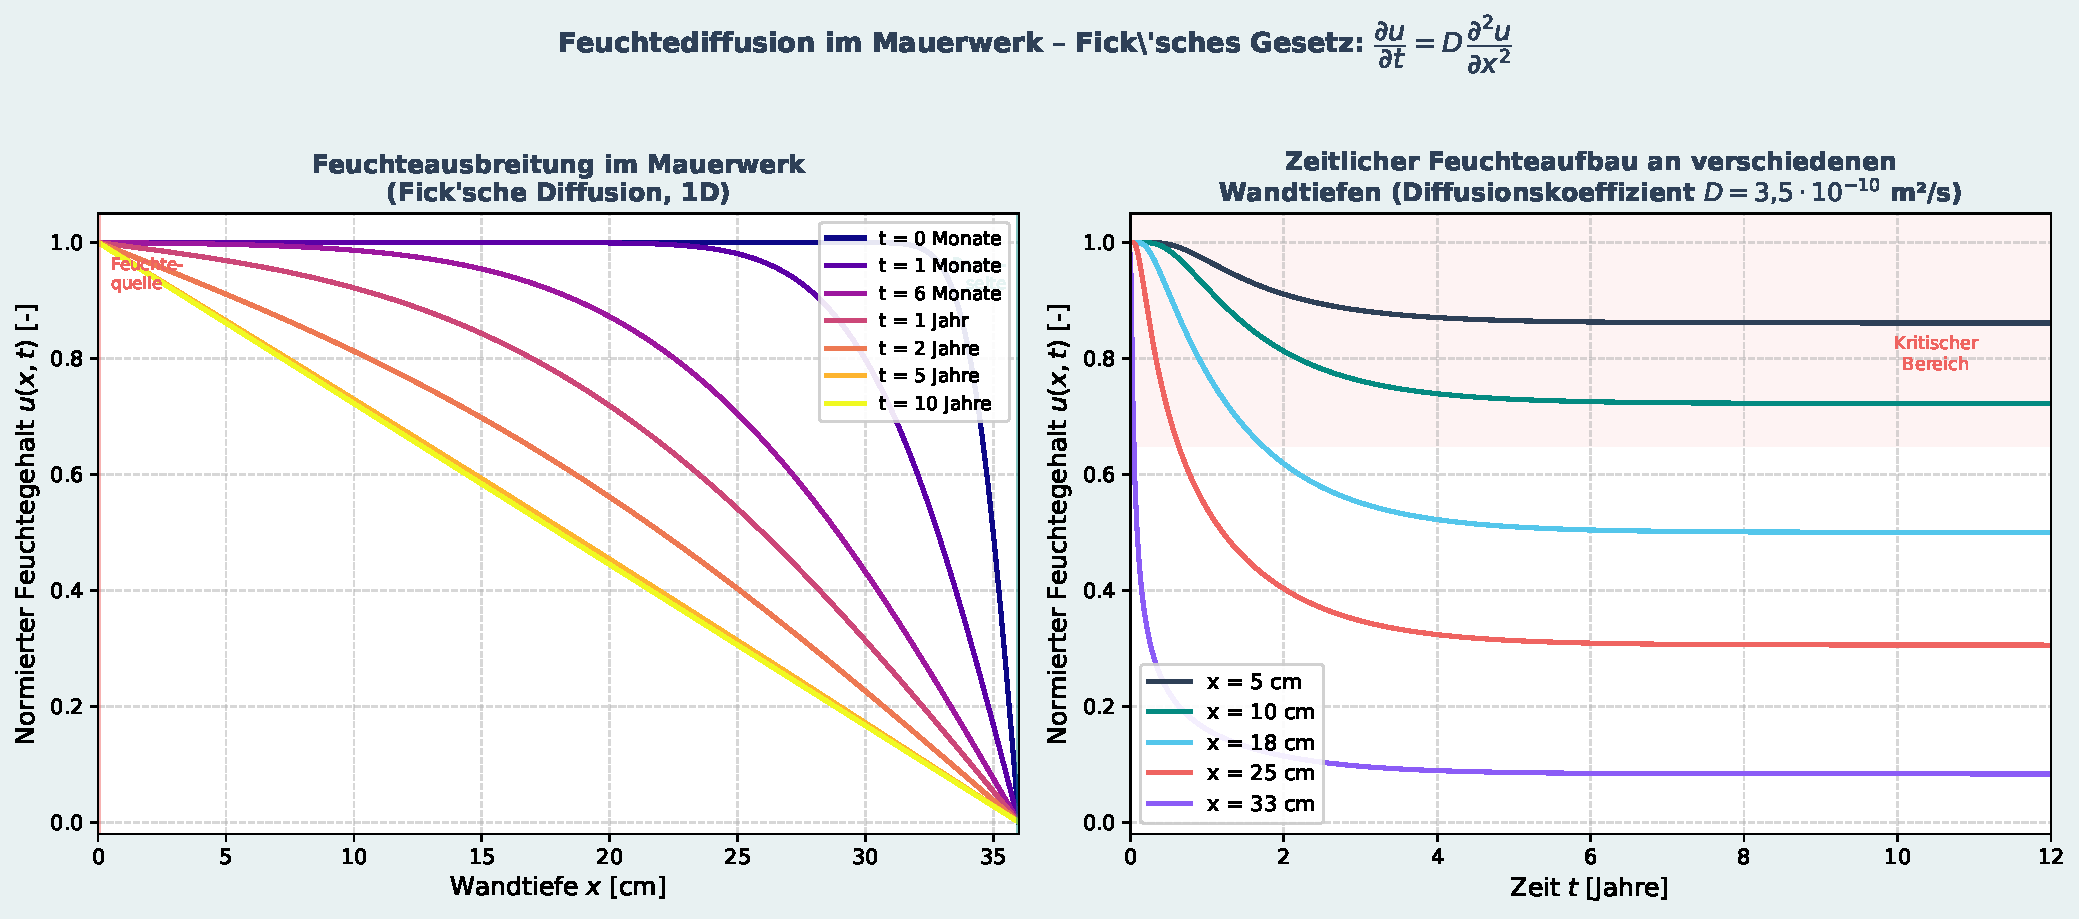
\includegraphics[width=\linewidth]{plot2_diffusion.pdf}
  \caption{%
    \textbf{Feuchtediffusion im Mauerwerk.}
    \textit{Links:} Normiertes Feuchtigkeitsprofil $u(x,t)$ im
    Wandquerschnitt zu verschiedenen Zeitpunkten (1 Monat bis 10 Jahre)
    nach Aktivierung der Feuchtebelastung. \textit{Rechts:} Zeitlicher
    Feuchteaufbau an f\"unf Messpositionen $(x = 5, 10, 18, 25, 33\ \mathrm{cm})$.
    Die orangefarbene Schraffur markiert den kritischen Feuchtebereich,
    ab dem Sch\"aden an Bausubstanz und Innenausstattung einsetzen.}
  \label{fig:diffusion}
\end{figure}

\subsection{Dampfdruckdiffusion und die Diffusionswiderstandszahl}

Der normierte Dampfdiffusionswiderstand (sd-Wert) einer Schicht ist:
\begin{equation}
  s_d = \mu \cdot d,
  \label{eq:sd}
\end{equation}
mit der Diffusionswiderstandszahl $\mu$ [-] (DIN EN ISO 10456) und der
Schichtdicke $d$ [\si{m}]. Im station\"aren Zustand ist der
Dampfpartialdruckverlauf $p(x)$ linear in der \"aquivalenten
Luftschichtdicke:
\begin{equation}
  p(x) = p_i - (p_i - p_e)\,\frac{s_d(x)}{s_{d,\mathrm{ges}}},
  \label{eq:partialdruck}
\end{equation}
wobei $p_i$ und $p_e$ die innen- und au\ss{}enseitigen Partialdr\"ucke
bezeichnen.

\begin{definition}[Kondensationsebene nach Glaser]
In einer mehrschichtigen Konstruktion tritt Kondensation auf, wenn
an einer Stelle $x^*$ der Partialdruck $p(x^*)$ den
S\"attigungsdampf\-druck $p_{\mathrm{sat}}(T(x^*))$ \"ubersteigt:
\begin{equation}
  p(x^*) > p_{\mathrm{sat}}(T(x^*)).
  \label{eq:kondensation}
\end{equation}
\end{definition}

Der S\"attigungsdampfdruck wird nach der Buck-Gleichung berechnet:
\begin{equation}
  p_{\mathrm{sat}}(T) = 611{,}21\,\exp\!\left(
    \frac{(18{,}678 - T/234{,}5)\,T}{257{,}14 + T}
  \right) \quad [\si{Pa}],
  \label{eq:psat}
\end{equation}
mit $T$ in \si{\celsius}.

\subsection{Taupunkttemperatur -- Magnus-Formel}

\begin{definition}[Taupunkttemperatur]
Die Taupunkttemperatur $T_d$ ist die Temperatur, auf die Luft mit
Temperatur $T$ und relativer Luftfeuchte $\phi$ abgek\"uhlt werden muss,
bis Kondensation einsetzt. Nach der Magnus-Formel gilt:
\begin{equation}
  T_d = \frac{b\,\alpha}{a - \alpha},
  \quad \alpha = \ln\phi + \frac{a\,T}{b + T},
  \label{eq:taupunkt}
\end{equation}
mit den Konstanten $a = 17{,}625$ und $b = \SI{243.04}{\celsius}$.
\end{definition}

\begin{korollar}[Kondensationsbedingung an Wandoberfl\"achen]
\label{kor:kondensation}
An einer Wandinnenoberfl\"ache mit Temperatur $T_{\mathrm{Wand}}$ setzt
Kondensation ein, sobald $T_{\mathrm{Wand}} < T_d(\phi_i, T_i)$,
wobei $T_i$ die Raumlufttemperatur und $\phi_i$ die relative
Raumluftfeuchte bezeichnen.
\end{korollar}

\begin{figure}[H]
  \centering
  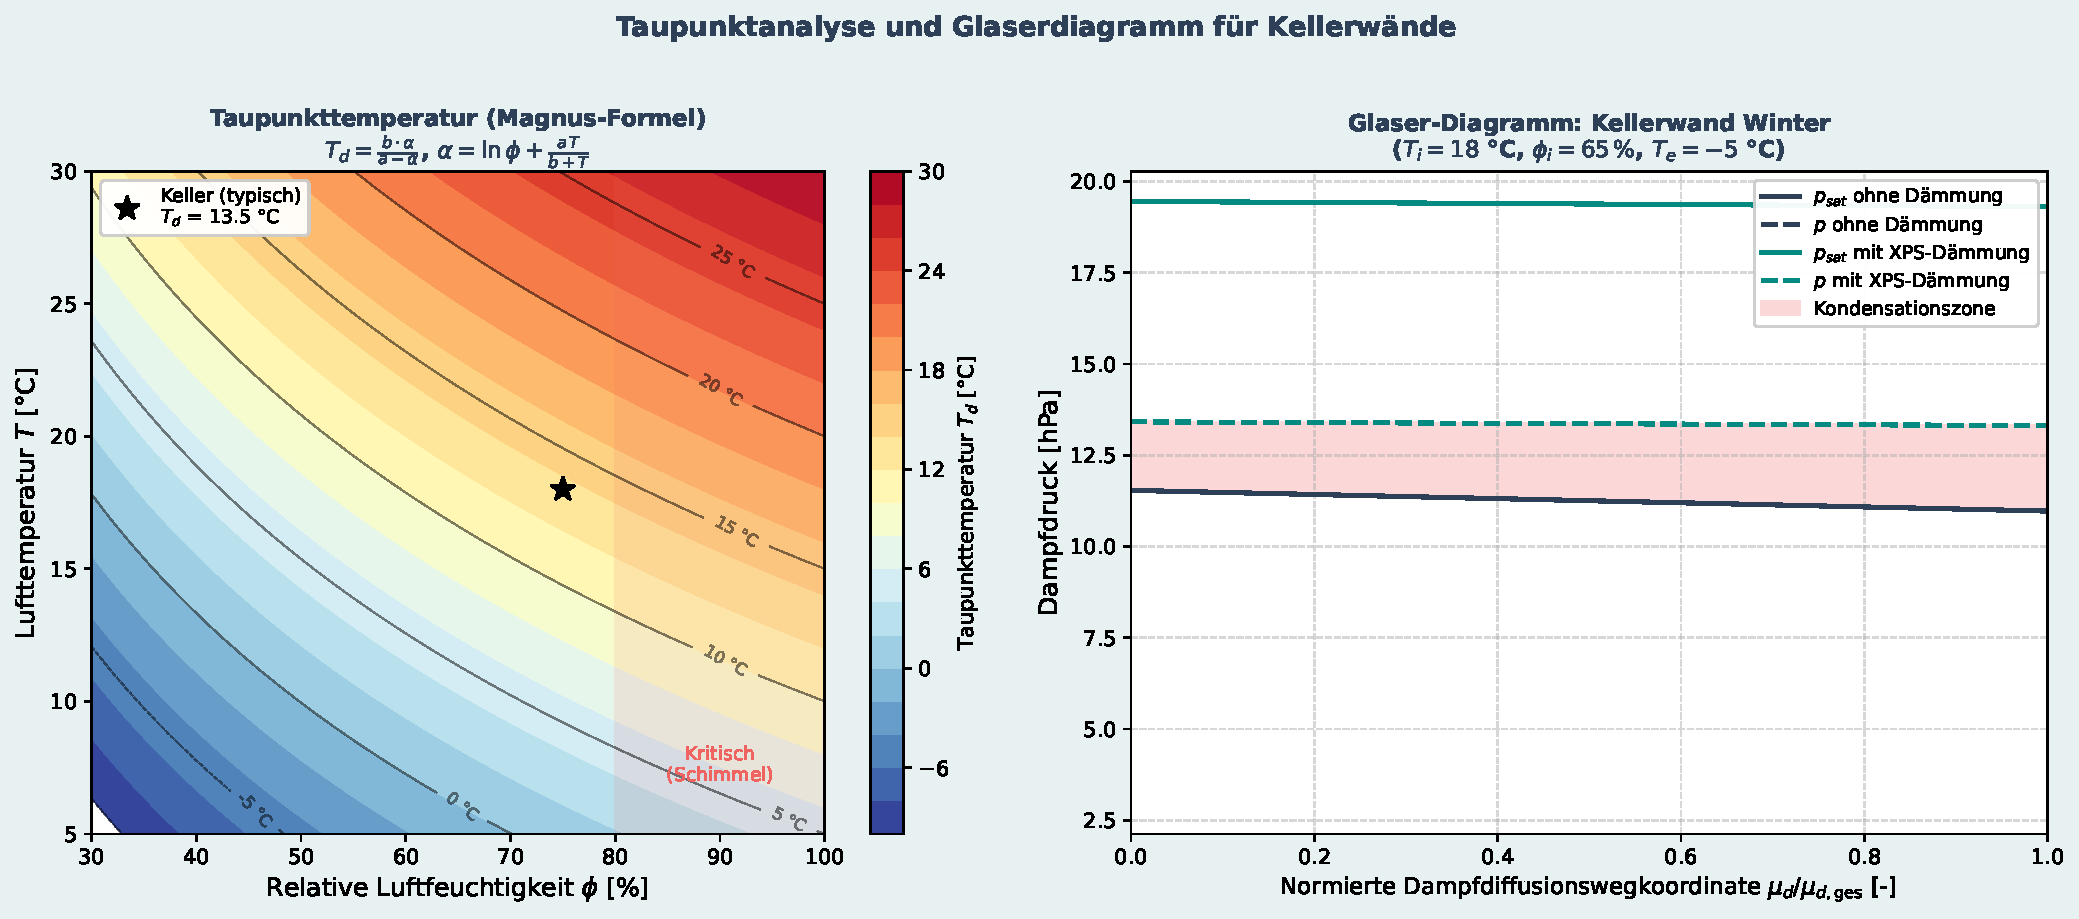
\includegraphics[width=\linewidth]{plot3_taupunkt.pdf}
  \caption{%
    \textbf{Taupunktanalyse und Glaserdiagramm.}
    \textit{Links:} Taupunkttemperatur $T_d$ nach \cref{eq:taupunkt}
    als Funktion von Raumtemperatur und relativer Luftfeuchtigkeit;
    der Stern markiert einen typischen Kellerbetriebspunkt.
    \textit{Rechts:} Glaserdiagramm f\"ur eine Kellerwand im Winter
    ($T_i = \SI{18}{\celsius}$, $\phi_i = 65\,\%$, $T_e = \SI{-5}{\celsius}$);
    ohne XPS-D\"ammung liegt der Partialdruck in der Kondensationszone
    \"uber dem S\"attigungsdampfdruck (orange schraffiert).}
  \label{fig:taupunkt}
\end{figure}

% =======================================================
\section{Ursachen von Feuchtesch\"aden}
\label{sec:ursachen}
% =======================================================

\subsection{Klassifikation der Feuchtigkeitsquellen}

\begin{definition}[Feuchtigkeitsklassen nach DIN 18533]
Die Norm DIN 18533 klassifiziert die Feuchteeinwirkung auf
erdber\"uhrte Bauteile in vier Klassen:
\begin{enumerate}[label=\textbf{W\arabic*}]
  \item Bodenfeuchte und nicht stauendes Sickerwasser
  \item Stauendes Sickerwasser
  \item Druckwasser bis zu \SI{3}{m} Einstaudauer
  \item Druckwasser mehr als \SI{3}{m} Einstaudauer
\end{enumerate}
\end{definition}

Im Wesentlichen lassen sich sechs Ursachenkategorien unterscheiden:

\subsubsection{Kapillarer Aufstieg}

In erdber\"uhrendem Mauerwerk ohne horizontale Sperrschicht steigt
Bodenfeuchtigkeit durch Kapillarkr\"afte auf. Die wirksame Steigh\"ohe
berechnet sich nach \cref{lem:steihoehe}. In Natursteinmauerwerk
mit mittleren Porenradien von $r \approx \SI{5}{\micro m}$ k\"onnen
Steigh\"ohen von \SI{3}{m} und mehr erreicht werden.

\subsubsection{Diffusion von Au\ss{}en}

Wasserdampf diffundiert bei Dampfdruckdifferenz durch Wandquerschnitte.
Die Diffusionsstromdichte berechnet sich aus \cref{eq:fick1}:
\begin{equation}
  j = -D_{\mu}\,\frac{\Delta p}{\Delta x}
    = \frac{p_i - p_e}{\mu\,d/(D_L)},
\end{equation}
mit der Luftdiffusivit\"at $D_L = \SI{2.56e-5}{m^2/s}$ bei
\SI{20}{\celsius} und \SI{1}{bar}.

\subsubsection{Druckwasser und Grundwasser}

Bei hohem Grundwasserstand oder nach Starkregenereignissen steht
Mauerwerk unter hydrostatischem Druck $p_h = \rho\,g\,h$. Eine
\SI{2}{m} Wassers\"aule erzeugt bereits $p_h \approx \SI{19.6}{kPa}$,
was die Saugspannungskapazit\"at der meisten Baustoffe \"ubersteigt.

\subsubsection{Kondensation an kalten Wandfl\"achen}

Entsprechend \cref{kor:kondensation} kondensiert Wasserdampf auf
Wandoberfl\"achen unterhalb des Taupunkts. Dieser Mechanismus tritt
besonders im Winter an Kellerau\ss{}enw\"anden auf, die durch den
Erdkontakt stark abgek\"uhlt werden.

\subsubsection{Bauwerksfeuchte und Restfeuchtigkeit}

Neubauten enthalten erhebliche Mengen Baufeuchte: Ein Kubikmeter
Beton enth\"alt bei der Herstellung ca. \SIrange{150}{180}{kg/m^3}
Anmachwasser, wovon nur ein Teil chemisch gebunden wird.
Die Austrocknungszeit $\tau_{\mathrm{tr}}$ l\"asst sich absch\"atzen:
\begin{equation}
  \tau_{\mathrm{tr}} \approx \frac{d^2}{2\,D_{\mathrm{eff}}}
  \label{eq:trocknung}
\end{equation}
und betr\"agt f\"ur eine \SI{25}{cm} Betonwand typischerweise
\SIrange{2}{5}{Jahre}.

\subsubsection{Undichte Leitungen und Havarie}

Defekte Wasserrohre, undichte Abl\"aufe und Dachabdichtungen stellen
zwar keine kontinuierliche, aber in der Schadensh\"ohe oft dominante
Feuchtigkeitsquelle dar.

\subsection{Wechselwirkungen und Synergiesch\"aden}

\begin{proposition}[Schimmelwachstumsbedingung nach Viitanen]
\label{prop:viitanen}
Das Schimmelwachstum setzt ein, wenn die relative Luftfeuchtigkeit
an der Oberfl\"ache die kritische Mindestfeuchte
\begin{equation}
  \phi_{\mathrm{krit}}(T) \approx
  \begin{cases}
    100\,\% & T < 0\,\si{\celsius}, \\
    (100 - 0{,}8\,T)\,\% & 0\,\si{\celsius} \le T < 20\,\si{\celsius}, \\
    (80 - 0{,}4\,(T-20))\,\% & T \ge 20\,\si{\celsius},
  \end{cases}
  \label{eq:phi_krit}
\end{equation}
\"ubersteigt. Der Schimmelindex $M$ nach Viitanen w\"achst mit der Rate
\begin{equation}
  \frac{\mathrm{d}M}{\mathrm{d}t} = k_1\,\cdot 0{,}035\,\cdot
  \frac{\phi - \phi_{\mathrm{krit}}}{1 - \phi_{\mathrm{krit}}}
  \cdot \frac{T + 5}{30}
  \quad [M/\mathrm{Tag}],
  \label{eq:viitanen}
\end{equation}
wobei $k_1 = 1$ f\"ur $T \ge \SI{5}{\celsius}$ und $k_1 = 0$ sonst.
Werte $M > 1$ indizieren sichtbares Schimmelwachstum.
\end{proposition}

\begin{figure}[H]
  \centering
  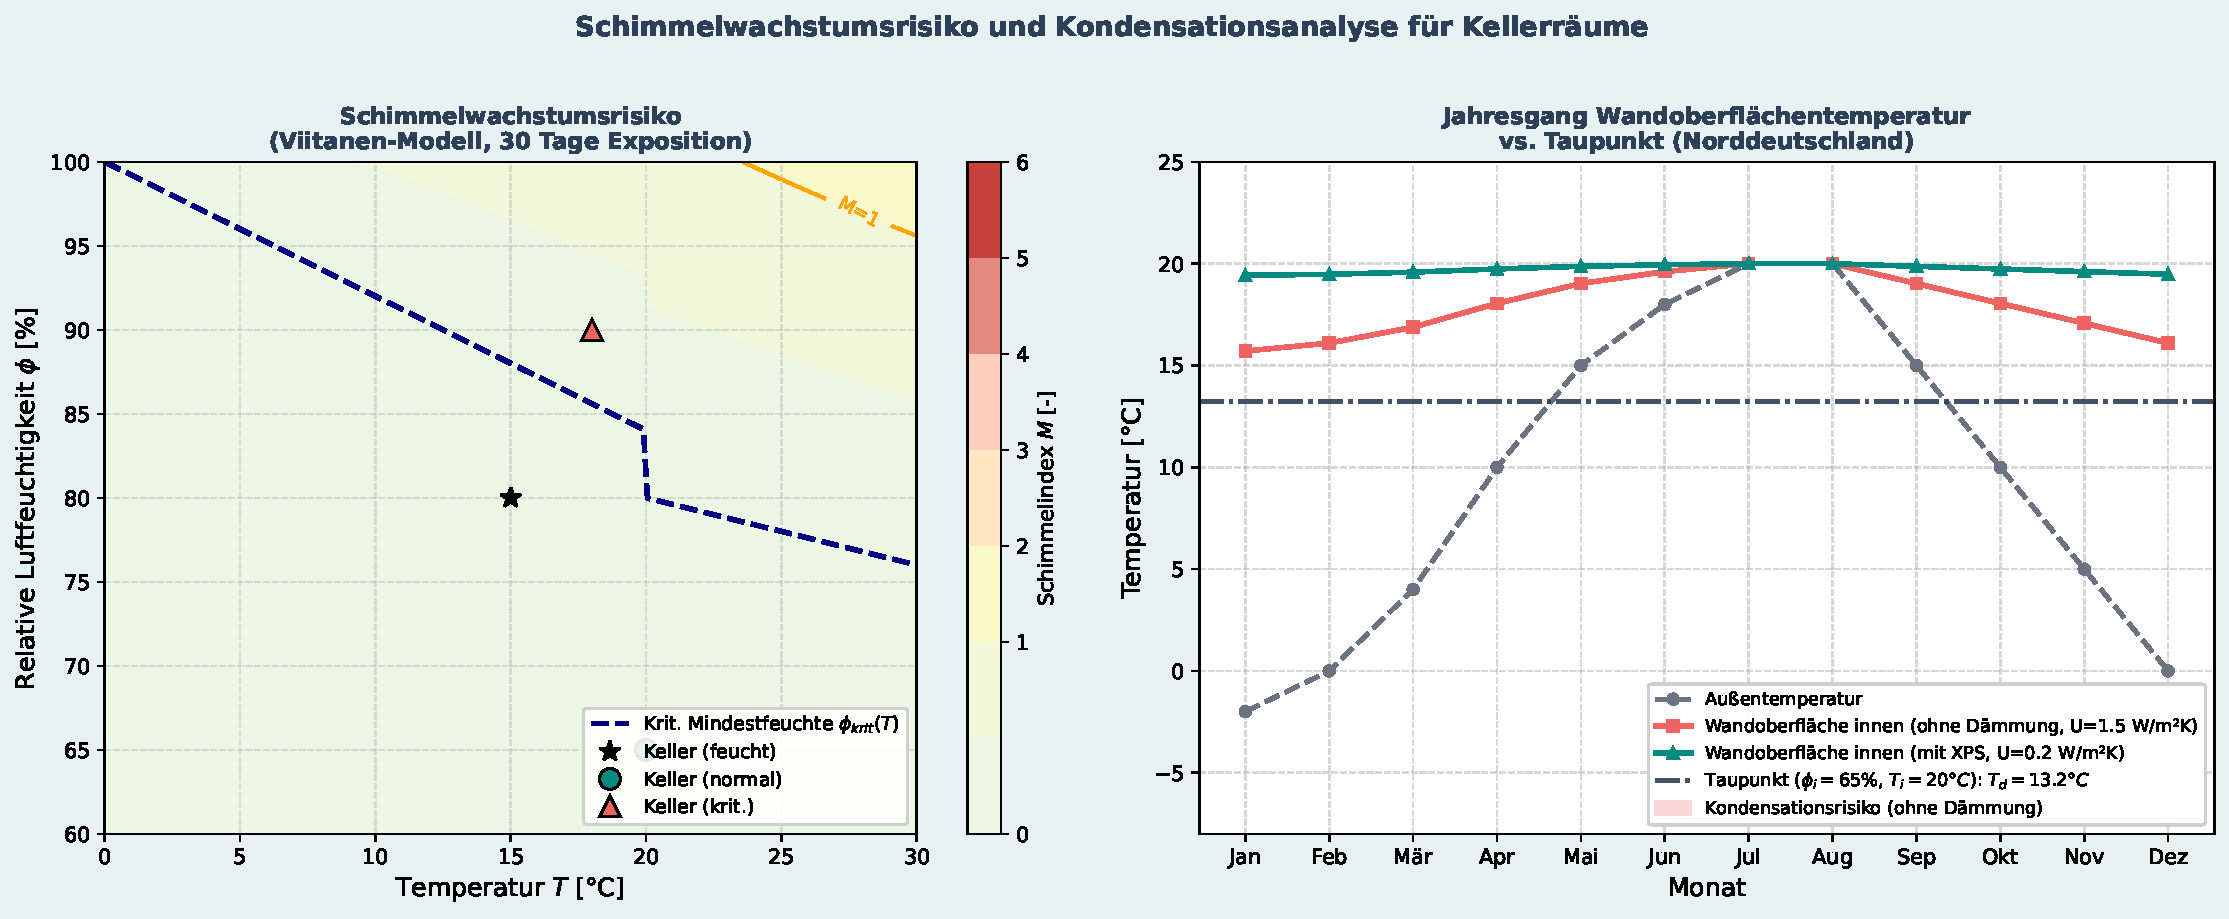
\includegraphics[width=\linewidth]{plot6_schimmel.pdf}
  \caption{%
    \textbf{Schimmelwachstumsrisiko und Kondensationsanalyse.}
    \textit{Links:} Schimmelindex $M$ nach \cref{prop:viitanen} als
    Funktion von Temperatur und relativer Feuchte (30~Tage Exposition);
    die gestrichelte Kurve markiert $\phi_{\mathrm{krit}}(T)$.
    \textit{Rechts:} Jahresgang der Wandoberfl\"achentemperatur (innen)
    f\"ur unged\"ammte Wand ($U = \SI{1.5}{W/m^2K}$) und XPS-ged\"ammte Wand
    ($U = \SI{0.20}{W/m^2K}$) im Vergleich zum Taupunkt
    ($\phi_i = 65\,\%$, $T_i = \SI{20}{\celsius}$); die orange Fl\"ache
    zeigt die Kondensationsperiode der unged\"ammten Wand.}
  \label{fig:schimmel}
\end{figure}

% =======================================================
\section{Pr\"aventive Ma\ss{}nahmen}
\label{sec:pravention}
% =======================================================

\subsection{Langfristige und baulich-konstruktive Pr\"avention}

\subsubsection{Au\ss{}enabdichtung und Perimeterd\"ammung}

Die normgerechte Au\ss{}enabdichtung (DIN 18533) ist die effektivste
langfristige Ma\ss{}nahme. Sie umfasst:
\begin{itemize}
  \item Voranstrich (Haftvermittler) auf dem Untergrund,
  \item Bitumen-Dickbeschichtung (PMBC) nach DIN 18533-3,
  \item XPS-Perimeterd\"ammplatten ($\lambda \le \SI{0.035}{W/mK}$,
        $\mu \ge 150$),
  \item Schutzlage (Noppenbahn oder Schutzvlies),
  \item Drainage aus kapillarbrechenden Kiesschichten oder
        Drainagerohren DN 100.
\end{itemize}

Der W\"armedurchgangskoeffizient der ged\"ammten Wand ergibt sich aus:
\begin{equation}
  U = \frac{1}{R_{si} + \sum_i d_i/\lambda_i + R_{se}},
  \label{eq:u-wert}
\end{equation}
mit dem Gesamtw\"armedurchgangswiderstand aller Schichten.

\subsubsection{Horizontale Sperrschicht}

Bei kapillarem Aufstieg ist eine horizontale Querschnittssperrung
unerl\"asslich. Materialien:
\begin{itemize}
  \item Bitumenbahnen (Typ V 60 S 4 nach DIN EN 13707),
  \item Kunststoffdichtungsbahnen (KDB, $s_d > \SI{100}{m}$),
  \item Stahlbleche (korrosionsgesch\"utzt),
  \item Injektionsmittel (als Alternative bei Bestandsbauten).
\end{itemize}

\subsubsection{Drainagesysteme}

Eine funktionierende Drainage h\"alt den hydrostatischen Druck auf
erdber\"uhrte W\"ande minimal. Der Darcysche Str\"omungsansatz beschreibt
den Wasserfluss durch die Drainageschicht:
\begin{equation}
  Q = -k_f\,A\,\frac{\Delta h}{\Delta l},
  \label{eq:darcy}
\end{equation}
mit dem Durchl\"assigkeitsbeiwert $k_f$ [\si{m/s}], der Querschnittsfl\"ache
$A$ [\si{m^2}] und dem hydraulischen Gradienten $\Delta h / \Delta l$.
Kiesf\"ullungen mit $k_f \ge \SI{e-3}{m/s}$ entsprechen der
Norm DIN EN 1610.

\subsection{Mittelfristige Ma\ss{}nahmen}

\subsubsection{Raumklimaoptimierung}

Die relative Raumluftfeuchte in Kellerr\"aumen sollte dauerhaft unter
60\,\% gehalten werden, um das Kondensationsrisiko nach
\cref{kor:kondensation} zu eliminieren. Hierf\"ur eignen sich:
\begin{itemize}
  \item Kontrollierte L\"uftung (Abluftsystem oder W\"armer\"uckgewinnung),
  \item Adsorptionsentfeuchter (Zeolith) f\"ur sehr kalte Keller,
  \item Kompressionsentfeuchter f\"ur Kellerr\"aume $> \SI{15}{\celsius}$.
\end{itemize}

\subsubsection{Dampfbremsfolien an Innenseiten}

Bei nicht zug\"anglicher Au\ss{}enseite kann eine Dampfbremse (sd-Wert
\SIrange{2}{50}{m}) die Diffusion von innen nach au\ss{}en begrenzen:
\begin{equation}
  s_d^{\mathrm{Bremse}} \ge \frac{p_i - p_e}{0{,}15\,p_{\mathrm{sat}}(T_e)}
    \cdot s_{d,\mathrm{Konstruktion}}.
\end{equation}

\begin{figure}[H]
  \centering
  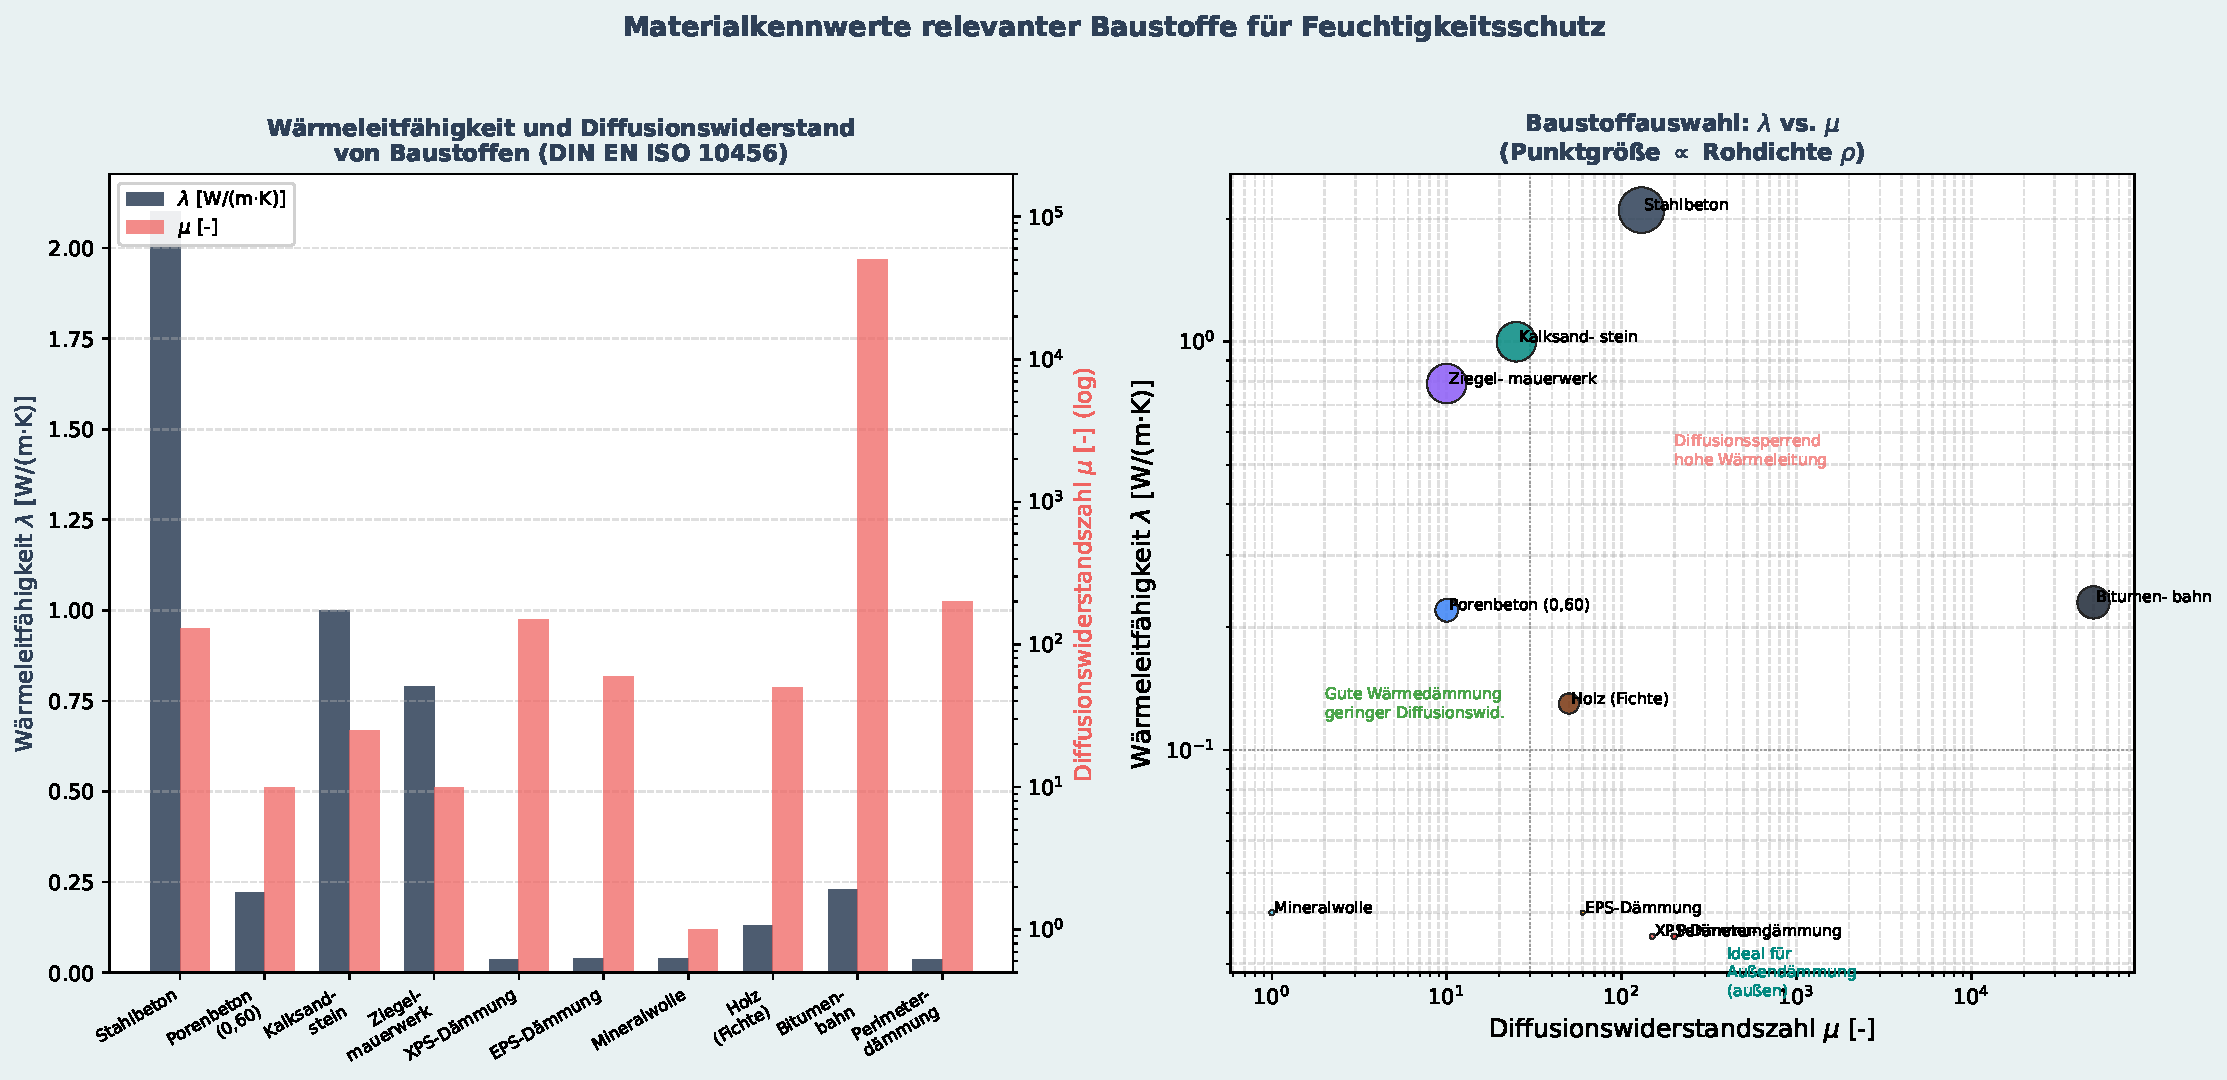
\includegraphics[width=\linewidth]{plot4_baustoffe.pdf}
  \caption{%
    \textbf{Materialkenndaten relevanter Baustoffe.}
    \textit{Links:} W\"armeleitf\"ahigkeit $\lambda$ (blau) und
    Diffusionswiderstandszahl $\mu$ (orange, logarithmisch) im Vergleich;
    Bitumenbahnen zeigen mit $\mu \approx 50\,000$ den h\"ochsten
    Diffusionswiderstand. \textit{Rechts:} Streudiagramm $\lambda$ vs.\ $\mu$
    (Punktgr\"o\ss{}e $\propto$ Rohdichte $\rho$); ideale D\"ammstoffe f\"ur
    Au\ss{}enanwendungen liegen im Bereich niedriger $\lambda$ und
    hoher $\mu$.}
  \label{fig:baustoffe}
\end{figure}

% =======================================================
\section{Sanierungsma\ss{}nahmen bei bestehenden Sch\"aden}
\label{sec:sanierung}
% =======================================================

\subsection{Schadensbewertung und Diagnostik}

Vor jeder Sanierung ist eine sorgf\"altige Schadensanalyse erforderlich.
Standardverfahren umfassen:
\begin{itemize}
  \item \textbf{CM-Messung} (Calciumcarbid-Methode): Feuchtegehalt
        $u_{\mathrm{CM}}$ [\%] in Baustoffen,
  \item \textbf{Schottsche Bohrlochmethode} zur Lokalisation der
        Sperrschicht,
  \item \textbf{Infrarot-Thermografie} zur Visualisierung von
        Temperaturinhomogenit\"aten (Norm EN 13187),
  \item \textbf{Radarverfahren} (GPR) zur zerst\"orungsfreien Detektion
        von Hohlr\"aumen und Rissen.
\end{itemize}

\subsection{Injektionsverfahren}

Das Injektionsverfahren schafft eine nachtr\"agliche horizontale oder
vertikale Sperrschicht. Das Injektionsmittel breitet sich im Porengef\"uge
aus und f\"ullt die Kapillaren hydrophob.

\begin{proposition}[Eindringtiefe nach Washburn]
\label{prop:washburn}
Die Eindringtiefe $l(t)$ eines Injektionsmittels (Viskosit\"at $\eta$,
Oberfl\"achenspannung $\gamma$, Kontaktwinkel $\theta$) in eine Pore mit
Radius $r$ gehorcht der Washburn-Gleichung:
\begin{equation}
  l(t) = \sqrt{\frac{r\,\gamma\,\cos\theta}{2\,\eta}\,t}.
  \label{eq:washburn}
\end{equation}
\end{proposition}

\begin{proof}
Aus dem Gleichgewicht zwischen Kapillardruck und viskosem Druckverlust
(Hagen-Poiseuille) folgt:
$\frac{2\gamma\cos\theta}{r} = \frac{8\eta\,l}{r^2}\,\frac{\mathrm{d}l}{\mathrm{d}t}$.
Separation und Integration ergibt $l^2 = \frac{r\gamma\cos\theta}{2\eta}\,t$,
woraus \cref{eq:washburn} folgt. 
\end{proof}

\subsection{Au\ss{}enabdichtung im Bestand}

Die nachtr\"agliche Freilegung und Abdichtung der Kellerau\ss{}enwand ist
die dauerhafteste L\"osung. Das Vorgehen:
\begin{enumerate}
  \item Freilegung der Au\ss{}enwand durch Erdarbeiten (Baggereinsatz),
  \item Mechanische Reinigung und Rissvorbehandlung,
  \item Aufbringen der Abdichtung (PMBC oder KDB nach DIN 18533),
  \item Schutzlage und D\"ammung (XPS),
  \item Drainage und Verf\"ullung.
\end{enumerate}

\subsection{Innenabdichtung als Notl\"osung}

Wenn die Au\ss{}enseite nicht zug\"anglich ist, k\"onnen mineralische
Dichtungsschl\"ammen (WU-Beton-Prinzip) oder flexible
Dichtungsschl\"ammen (FDS II) auf der Innenseite aufgebracht werden.
Diese nehmen den Wasserdruck von innen auf, l\"osen aber die Ursache
nicht und sind daher als \"Ubergangsl\"osung zu werten.

\subsection{Sanierputzsysteme}

Sanierputze (WTA Merkblatt 2-9) nehmen kapillar eingedrungene
Feuchtigkeit auf und speichern hygroskopische Salze,
ohne deren Migration an die Oberfl\"ache zu erm\"oglichen. Sie bestehen
aus einer Unterputzlage (Porenvolumen $> 40\,\%$) und einem
Oberputz mit hydrophobierenden Zus\"atzen.

\begin{figure}[H]
  \centering
  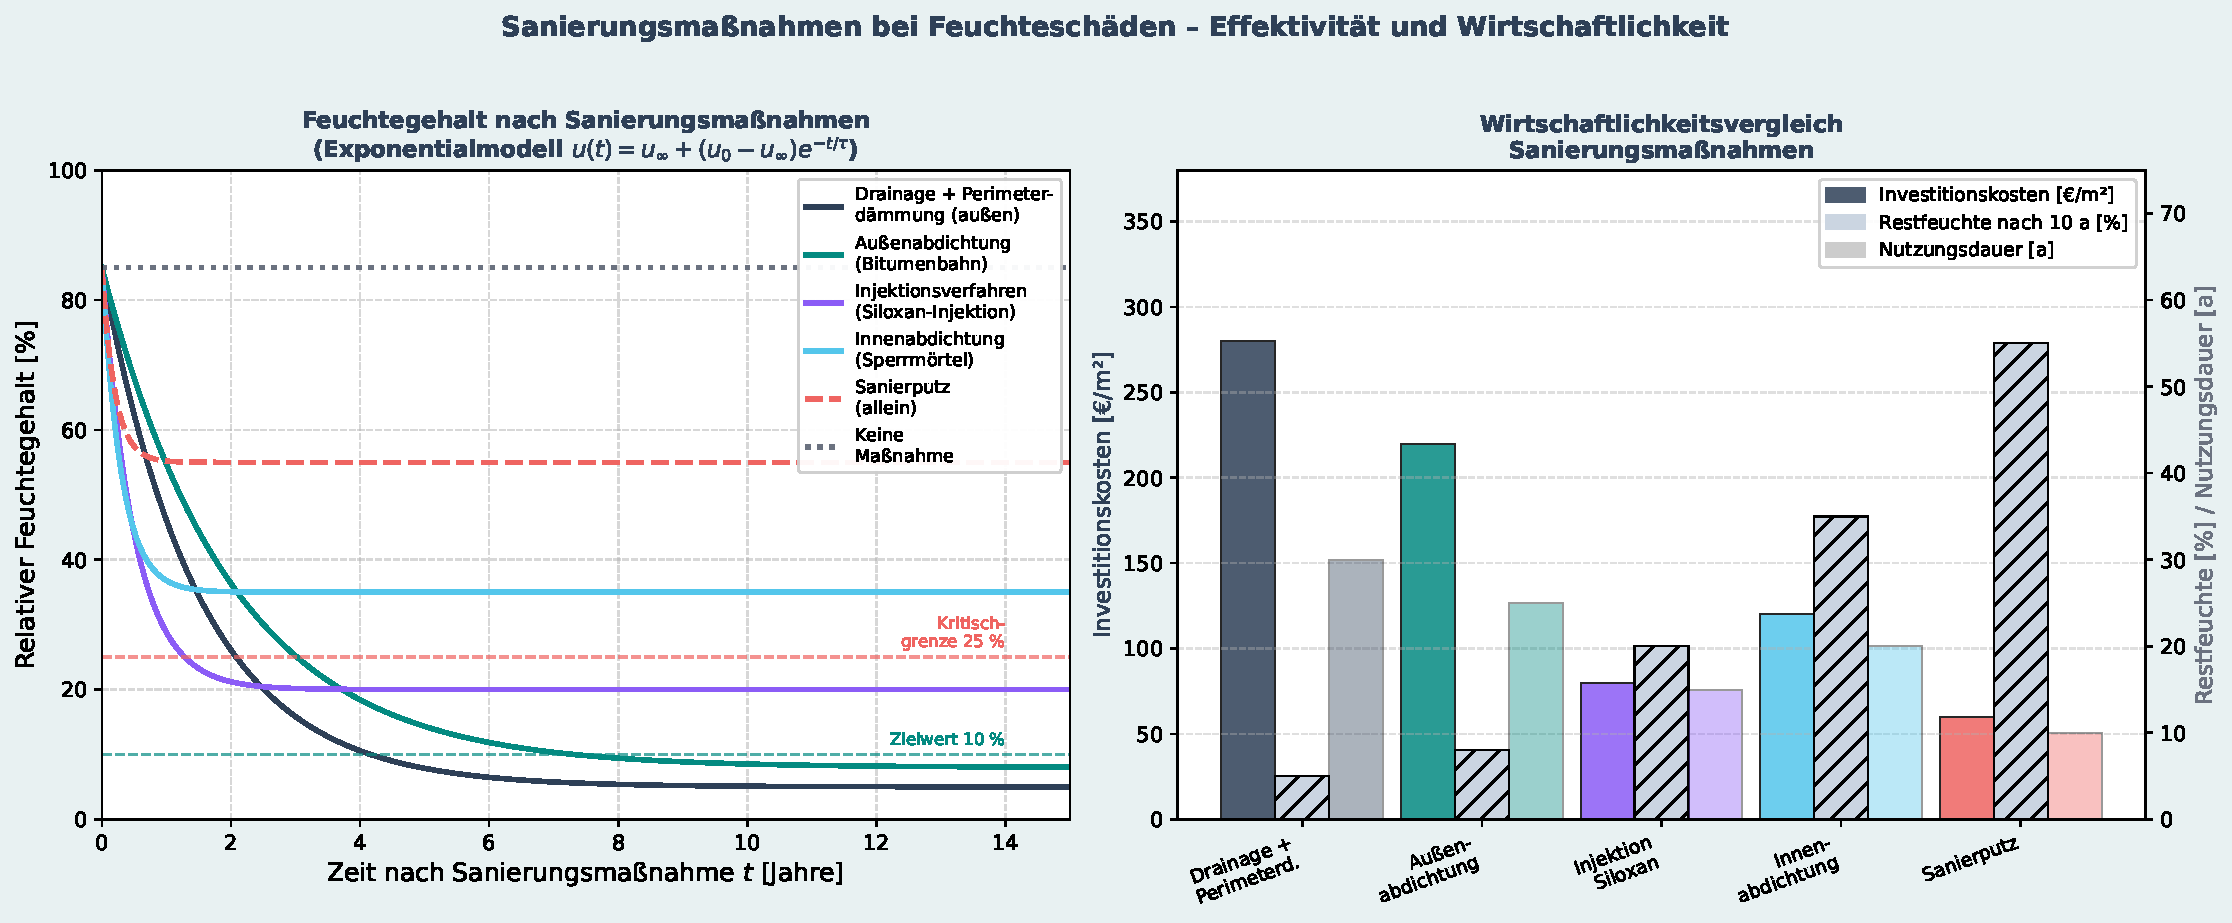
\includegraphics[width=\linewidth]{plot5_sanierung.pdf}
  \caption{%
    \textbf{Effektivit\"at und Wirtschaftlichkeit von Sanierungsma\ss{}nahmen.}
    \textit{Links:} Zeitlicher Verlauf des Feuchtegehalts nach
    verschiedenen Sanierungsma\ss{}nahmen (Exponentialmodell
    $u(t) = u_\infty + (u_0 - u_\infty)\,e^{-t/\tau}$); die gestrichelten
    Linien markieren Zielwert ($10\,\%$) und Kritischgrenze ($25\,\%$).
    \textit{Rechts:} Vergleich von Investitionskosten [EUR/m²],
    Restfeuchtegehalt nach 10~Jahren und Nutzungsdauer der Ma\ss{}nahme.}
  \label{fig:sanierung}
\end{figure}

\subsection{Bewertungsmatrix}

\begin{longtable}{>{\bfseries}p{3.2cm}p{1.8cm}p{1.8cm}p{2.0cm}p{2.5cm}}
  \caption{Vergleich von Sanierungsma\ss{}nahmen nach DIN 18533 und WTA-Merkblatt.}
  \label{tab:massnahmen}\\
  \toprule
  Ma\ss{}nahme & Kosten [EUR/m²] & Nutzungsd. [a] & Restfeuchte [Gew-\%] & Anwendbarkeit \\
  \midrule
  \endfirsthead
  \toprule
  Ma\ss{}nahme & Kosten [EUR/m²] & Nutzungsd. [a] & Restfeuchte [Gew-\%] & Anwendbarkeit \\
  \midrule
  \endhead
  \bottomrule
  \endfoot
  Drainage + Perimeter-\newline d\"ammung (au\ss{}en) & 280 & 30 & 5 & Neubau, Bestand \\
  Au\ss{}enabdichtung\newline (Bitumenbahn, KDB) & 220 & 25 & 8 & Neubau, Bestand \\
  Injektionsverfahren\newline (Siloxan, Acrylat) & 80 & 15 & 20 & Bestand \\
  Innenabdichtung\newline (mineralisch/flexibel) & 120 & 20 & 35 & Bestand, Not \\
  Sanierputzsystem\newline (WTA 2-9) & 60 & 10 & 55 & Bestand, tempor\"ar \\
\end{longtable}

% =======================================================
\section{Ergebnisse und Diskussion}
\label{sec:ergebnisse}
% =======================================================

Die physikalischen Analysen dieser Arbeit zeigen drei wesentliche Befunde:

\textbf{(1) Kapillartransport dominiert bei erdber\"uhrtem Mauerwerk.}
Nach \cref{lem:steihoehe} k\"onnen Steigh\"ohen von mehreren Metern
auftreten, sofern keine horizontale Sperrschicht vorhanden ist.
\Cref{fig:kapillardruck} belegt, dass bereits Poren mit
$r = \SI{1}{\micro m}$ Dr\"ucke von \"uber \SI{0.14}{MPa} erzeugen,
was Sperrm\"orteln ohne Rissfreiheit entgegenwirkt.

\textbf{(2) Diffusionsprozesse sind langsam aber persistent.}
Aus \cref{thm:fourier} und \cref{fig:diffusion} ergibt sich,
dass die Feuchteausbreitung in einer \SI{36}{cm} Betonwand \"uber
Jahrzehnte anh\"alt. Die charakteristische Diffusionszeit betr\"agt
$\tau_D = L^2/(\pi^2 D) \approx \SI{11.7}{Jahre}$ f\"ur die angegebenen
Parameter. Ohne Abdichtung stellt sich ein station\"ares Profil ein,
das die Wand dauerhaft durchfeuchtet.

\textbf{(3) Kondensation tritt jahreszeitlich auf.}
Das Glaserdiagramm in \cref{fig:taupunkt} zeigt, dass an unged\"ammten
Kellerau\ss{}enw\"anden ($U = \SI{1.5}{W/m^2K}$) bei norddeutschem Klima
in den Monaten November bis M\"arz Kondensation an der Innenwandfl\"ache
auftreten kann (\cref{fig:schimmel}). XPS-D\"ammung ($U = \SI{0.20}{W/m^2K}$)
eliminiert dieses Risiko vollst\"andig.

% =======================================================
\section{Schlussfolgerungen}
\label{sec:fazit}
% =======================================================

Feuchtesch\"aden an W\"anden und Kellern sind physikalisch vollst\"andig
beschreibbar und damit auch beherrschbar. Die vorliegende Arbeit
demonstriert, dass die Kombination von:
\begin{enumerate}
  \item au\ss{}enseitiger Perimeterd\"ammung mit kapillarbrechendem Drainagesystem,
  \item normgerechter Abdichtung nach DIN 18533,
  \item raumklimatischer Kontrolle ($\phi_i < 60\,\%$)
\end{enumerate}
praktisch alle Feuchteschadensursachen dauerhaft ausschlie\ss{}t.

Die Wirtschaftlichkeitsanalyse in \cref{fig:sanierung} und
\cref{tab:massnahmen} belegt, dass die kostenintensivere Au\ss{}ensanierung
mit ca.~\SI{280}{EUR/m^2} \"uber eine Nutzungsdauer von 30~Jahren
deutlich kosteng\"unstiger ist als wiederholte Innenma\ss{}nahmen.

% =======================================================
\section{Ausblick}
\label{sec:ausblick}
% =======================================================

Die vorliegende Arbeit schafft eine solide physikalische Grundlage
f\"ur das Verst\"andnis und die Behandlung von Feuchtesch\"aden.
Gleichwohl bestehen zahlreiche offene Forschungs- und Entwicklungsfelder,
die im Folgenden ausf\"uhrlich beschrieben werden.

\subsection{Numerische Simulation und digitale Zwillinge}

Die analytischen L\"osungen dieser Arbeit basieren auf vereinfachten
Annahmen wie konstanten Materialparametern, linearen Randbedingungen
und eindimensionaler Geometrie. Reale Bauwerke sind dreidimensional,
anisotrop und weisen zeitver\"anderliche Randbedingungen auf.

Zuk\"unftige Arbeiten sollten vollst\"andige 3D-Finite-Elemente-Simulationen
des gekoppelten W\"arme-Feuchte-Transports implementieren,
wie sie durch die HAM-Methode (Heat, Air, Moisture) beschrieben wird
und in Softwaretools wie WUFI Pro oder Delphin bereits realisiert ist.
Die Kopplung an digitale Zwillinge (Digital Twins) realer Geb\"aude
w\"urde die kontinuierliche Prognose von Feuchtezust\"anden anhand von
Sensordaten erm\"oglichen. Hierf\"ur werden IoT-Sensornetze in W\"anden
ben\"otigt, die Temperatur, Feuchte und Salzgehalt mit r\"aumlicher
Aufl\"osung erfassen.

Ein wichtiger Schritt ist die Implementierung hygrothermischer
R\"uckkopplungseffekte: Feuchtigkeit ver\"andert die W\"armeleitf\"ahigkeit
$\lambda$ erheblich (Wasser: $\lambda = \SI{0.6}{W/mK}$,
Luft: $\lambda = \SI{0.025}{W/mK}$), was bei h\"oheren Feuchtegehalten
die Isolationswirkung stark verschlechtert. Diese Nichtlinearit\"at
$\lambda = \lambda(u)$ muss in zuk\"unftigen Modellen ber\"ucksichtigt werden.

\subsection{Maschinelles Lernen und KI-gest\"utzte Schadensdiagnose}

Die Kombination von hygrothermischen Sensordaten mit maschinellen
Lernverfahren er\"offnet neue M\"oglichkeiten der Fr\"uhschadenserkennung.
Neuronale Netzwerkmodelle (z.\,B. LSTM-Netze f\"ur Zeitreihenanalyse)
k\"onnten aus historischen Messdaten trainiert werden, um Anomalien
im Feuchteregime zu detektieren, bevor sichtbare Sch\"aden auftreten.

Besonders vielversprechend ist der Einsatz von Convolutional Neural
Networks (CNN) zur Analyse von Infrarot-Thermografieaufnahmen.
Hierdurch k\"onnten Feuchtestellen automatisch lokalisiert und
quantifiziert werden, ohne dass manuelle Auswertung durch Sachverst\"andige
erforderlich ist. Transferlernen auf Basis vortrainierter Bildklassifikations-
modelle (z.\,B. ResNet, EfficientNet) bietet sich dabei an.

Reinforcement-Learning-Ans\"atze k\"onnten zuk\"unftig optimale
L\"uftungsstrategien zur Vermeidung von Kondensation in Echtzeit
berechnen, unter Ber\"ucksichtigung von Energieverbrauch,
Komfort und Feuchtebelastung.

\subsection{Neue Materialien und Nanokomposite}

Die Materialentwicklung bietet enormes Potential. Folgende Entwicklungen
sind besonders relevant:

\textbf{Hydrophobe Beton-Additive:} Siloxan-basierte Additive, die
direkt in die Betonmischung eingebracht werden, verleihen dem gesamten
Bauteil kapillarbremerische Eigenschaften. Aktuelle Forschungsarbeiten
untersuchen die Langzeitbest\"andigkeit solcher Systeme \"uber
Zeitr\"aume $> 50$ Jahre.

\textbf{Selbstheilende Materialien:} Bakterienbasierte Selbstheilungsbetone
(z.\,B. basierend auf \textit{Bacillus subtilis}) schlie\ss{}en Mikrorisse
durch biogene Calcit-Ausf\"allung. Erste Feldversuche zeigen
Rissschlie\ss{}ungsraten von bis zu 0{,}8~mm Rissweite, was die
Feuchteaufnahme durch Risskorrosion deutlich reduziert.

\textbf{Aerogel-D\"ammstoffe:} Silica-Aerogele erreichen
W\"armeleitf\"ahigkeiten v. $\lambda < \SI{0.015}{W/mK}$ bei sehr
niedrigen $\mu$-Werten ($\mu \approx 3$). Zuk\"unftige Entwicklungen
zielen auf mechanisch robuste Aerogel-Verbundplatten, die f\"ur
Perimeterd\"ammung geeignet sind.

\textbf{Phasen\"anderungsmaterialien (PCM):} Die Integration von
Paraffin-Mikrokapseln in Putzm\"ortel erh\"oht die thermische Tr\"agheit
der Wandoberfl\"ache, wodurch Temperaturschwankungen -- und damit
das Kondensationsrisiko -- ged\"ampft werden.

\subsection{Energetische Sanierung und Feuchteschutz -- Synergien}

Die Versch\"arfung der Anforderungen an W\"armed\"ammung im GEG 2024
birgt das Risiko, dass energetische Sanierungsma\ss{}nahmen ohne
gleichzeitige Feuchtebetrachtung neue Sch\"aden erzeugen
(Innend\"ammung, W\"armebr\"ucken, Tauwasserprobleme). Zuk\"unftige
Forschungsarbeit sollte:
\begin{itemize}
  \item Ganzheitliche Optimierungsmodelle entwickeln, die Energieeffizienz
        und Feuchteschutz simultan optimieren,
  \item Neue Regelwerke (DIN, EN) erarbeiten, die explizit
        hygrothermische Nachweise f\"ur alle Sanierungsszenarien fordern,
  \item Die Wechselwirkungen von Innend\"ammung mit historischen
        Mauerwerksstrukturen systematisch quantifizieren.
\end{itemize}

\subsection{Klimaanpassung und Extremwetterereignisse}

Klimaprojektionen (DWD, IPCC AR6) zeigen f\"ur Deutschland bis 2100:
intensivere Starkregenereignisse ($+30\,\%$ Intensit\"at),
h\"aufigere Fr\"uhjahrsfrost-Tau-Wechsel sowie regional sinkende
Grundwasserspiegel im Sommer bei steigendem Druckwasserrisiko
im Winter. Die Konsequenzen f\"ur den Feuchteschutz sind erheblich:
\begin{itemize}
  \item Drainagesysteme m\"ussen auf h\"ohere Spitzenabfl\"usse ($Q_{\max}$)
        ausgelegt werden (DIN EN 752),
  \item Abdichtungsmaterialien m\"ussen erh\"ohte Frost-Tau-Wechselbest\"andigkeit
        aufweisen (Pr\"ufnorm EN 1108),
  \item Geb\"audemodellierungen m\"ussen mit Klimaprojektionsdaten
        (RCP 4.5, RCP 8.5) als Randbedingungen durchgef\"uhrt werden.
\end{itemize}

\subsection{Normung und rechtliche Rahmenbedingungen}

Trotz bestehender Normen (DIN 18533, DIN 4108, WTA-Merkbl\"atter)
gibt es erhebliche L\"ucken: Es fehlen einheitliche Bewertungsma\ss{}st\"abe
f\"ur den Feuchtegehalt im Bestand, keine klaren Grenzwerte f\"ur
zul\"assige Restfeuchte in Wohnr\"aumen (nur Empfehlungen nach WTA 4-11),
und die Schnittstelle zwischen Energieeinsparverordnung und
hygrothermischen Nachweisverfahren ist unzureichend definiert.

Zuk\"unftige Normenarbeit sollte einen verpflichtenden hygrothermischen
Gesamtnachweis (analog zum OIB-Richtlinien-Ansatz in \"Osterreich)
f\"ur alle Kellergeschoss-Sanierungen in Deutschland einf\"uhren.

\subsection{Gesellschaftliche und wirtschaftliche Dimension}

Rund 70\,\% des deutschen Wohngeb\"audebestands wurde vor 1979 errichtet,
vor Einf\"uhrung der ersten W\"armeschutzverordnung. Ein erheblicher Teil
dieser Geb\"aude weist unzureichende Abdichtungen und fehlende
Perimeterd\"ammung auf. Hochrechnungen zeigen ein Sanierungsvolumen
von \"uber \SI{200}{\text{Mrd.}EUR} f\"ur den feuchtigkeitsbezogenen
Geb\"audeschutz in Deutschland.

F\"orderprogramme (KfW-Sanierungskredit 261, BAFA-Zuschuss) decken
derzeit nur einen Teil der Sanierungskosten. Zuk\"unftige politische
Ma\ss{}nahmen sollten Anreize schaffen, Feuchtigkeitssanierungen mit
energetischen Ma\ss{}nahmen zu koppeln und so Synergieeffekte zu nutzen.

\subsection{Zusammenfassung des Ausblicks}

Tabelle~\ref{tab:ausblick} fasst die wichtigsten Forschungs- und
Entwicklungsfelder mit Zeithorizont und Potenzial zusammen.

\begin{longtable}{>{\bfseries}p{4.0cm}p{3.0cm}p{2.5cm}p{3.0cm}}
  \caption{Forschungs- und Entwicklungsfelder im Feuchteschutz.}
  \label{tab:ausblick}\\
  \toprule
  Themenfeld & Methoden & Zeithorizont & Potenzial \\
  \midrule
  \endfirsthead
  \toprule
  Themenfeld & Methoden & Zeithorizont & Potenzial \\
  \midrule
  \endhead
  \bottomrule
  \endfoot
  3D-Simulation HAM & FEM, CFD & 2--5 Jahre & Sehr hoch \\
  Digitale Zwillinge & IoT, BIM & 3--7 Jahre & Hoch \\
  KI-Schadensdiagnose & CNN, LSTM & 2--4 Jahre & Sehr hoch \\
  Selbstheilende Materialien & Biotechnologie & 5--15 Jahre & Hoch \\
  Aerogel-Perimeterd. & Nanomaterialien & 3--8 Jahre & Mittel--Hoch \\
  PCM-Wandsysteme & Thermochemie & 2--5 Jahre & Mittel \\
  Klimaangepasste Normen & Normungsarbeit & 3--10 Jahre & Sehr hoch \\
  Politische F\"orderprogramme & Gesetzgebung & 1--3 Jahre & Hoch \\
\end{longtable}

% =======================================================
% Literaturverzeichnis
% =======================================================
\begin{thebibliography}{99}

\bibitem{DIN18533}
DIN Deutsches Institut f\"ur Normung e.\,V.\ (2017).
\textit{DIN 18533: Abdichtung von erdber\"uhrten Bauteilen -- Teile 1--3}.
Beuth Verlag, Berlin.

\bibitem{DIN4108}
DIN Deutsches Institut f\"ur Normung e.\,V.\ (2021).
\textit{DIN 4108-2: W\"armeschutz und Energie-Einsparung in Geb\"auden --
Mindestanforderungen an den W\"armeschutz}.
Beuth Verlag, Berlin.

\bibitem{ISO10456}
DIN EN ISO 10456 (2010).
\textit{Baustoffe und Bauprodukte -- W\"arme- und feuchtetechnische
Eigenschaften -- Tabellierte Bemessungswerte und Verfahren zur Bestimmung
der w\"armeschutztechnischen Nenn- und Bemessungswerte}.
Beuth Verlag, Berlin.

\bibitem{WTA}
Wissenschaftlich-Technische Arbeitsgemeinschaft f\"ur Bauwerkserhaltung
und Denkmalpflege e.\,V.\ (2018).
\textit{WTA-Merkblatt 4-11-18/D: Messung der Feuchte von Mauerwerk}.
WTA Publications, M\"unchen.

\bibitem{Glaser1958}
Glaser, H. (1958).
Graphisches Verfahren zur Untersuchung von Diffusionsvorg\"angen.
\textit{K\"altetechnik}, 10(10), 345--349.

\bibitem{Viitanen1994}
Viitanen, H. (1994).
\textit{Factors affecting the development of mould and brown rot decay
in wooden material and wooden structures -- effect of humidity,
temperature and exposure time}.
Swedish University of Agricultural Sciences, Uppsala.

\bibitem{Magnus1844}
Magnus, G. (1844).
Versuche \"uber die Dampfspannungen des Wassers und einiger anderer
Fl\"ussigkeiten.
\textit{Annalen der Physik}, 137(2), 225--247.

\bibitem{Young1805}
Young, T. (1805).
An essay on the cohesion of fluids.
\textit{Philosophical Transactions of the Royal Society of London},
95, 65--87.

\bibitem{Fick1855}
Fick, A. (1855).
\"Uber Diffusion.
\textit{Annalen der Physik}, 170(1), 59--86.

\bibitem{Washburn1921}
Washburn, E.\,W. (1921).
The dynamics of capillary flow.
\textit{Physical Review}, 17(3), 273--283.

\bibitem{Darcy1856}
Darcy, H. (1856).
\textit{Les fontaines publiques de la ville de Dijon}.
Dalmont, Paris.

\bibitem{IPCC2021}
IPCC (2021).
\textit{Climate Change 2021: The Physical Science Basis.
Contribution of Working Group I to the Sixth Assessment Report}.
Cambridge University Press, Cambridge.

\bibitem{Kuenzel1995}
K\"unzel, H.\,M. (1995).
\textit{Simultaneous heat and moisture transport in building components --
one- and two-dimensional calculation using simple parameters}.
IRB Verlag, Stuttgart.

\bibitem{DIN1610}
DIN EN 1610 (2015).
\textit{Verlegung und Pr\"ufung von Abwasserleitungen und -kan\"alen}.
Beuth Verlag, Berlin.

\end{thebibliography}

\end{document}